\textbf{Implementación de la tarjeta de desarrollo e humano-máquina}

Para el funcionamiento del software del sistema mecatrónico, se implementó una tarjeta ESP32, la cual se montó en un protoboard para realizar las conexiones necesarias para el funcionamiento del circuito electrónico principal. 

Para la implementación, se realizo un código (Apéndice \ref{Ap:Codigo_completo}) en lenguaje C a través de la interfaz de Arduino 2.0. El código está formado por 4 hilos, que son diferentes rutinas que se ejecutan de manera simultanea dentro de los procesadores del microcontrolador.

Las diferentes subrutinas se comunican por medio de banderas internas, declaradas al interior del código para coordinar a los distintos actuadores. 

El hilo principal, se encarga de recibir la señal  de inicio al proceso de compostaje, arrancando la interfaz, también se encarga de iniciar los registros necesarios para verificar el avance del tiempo. 

Un segundo hilo es el encargado de registrar el tiempo general del proceso, sumando una unidad a un registro llamado "Segundos" cada vez que se realiza una pausa con un periodo de 1 segundo. En este mismo hilo, se realiza una secuencia de instrucciones para agrupar los minutos y las horas para al final, cuando se cumpla el ciclo total de 72 horas, mandará una bandera que indique el fin del proceso y detenga las tareas de los actuadores.

El tercer hilo se encarga de coordinar los proceso de aireación, los cuales activarán el eje de aireación junto al sistema de ventilación por 10 minutos cada 3 horas, para mezclar y oxigenar los residuos.

El último hilo, se encarga de leer los valores recopilados de los sensores de DHT11 (Humedad) y el DS18B20 (Temperatura) y realizar las etapas de control de encendido de los procesos de regulación de temperatura y regulación de humedad.

Para poder interactuar con el dispositivo, dentro del hilo principal, se ha implementado una interfaz (figura \ref{fg:cto_interfaz_fisico}), aquí se han colocado los botones (Figura \ref{fg:botones_imp}), para permitir que el usuario demande cierto tipo de información que estará disponible por medio de un menú.

\begin{figure}[h]
            \centering
            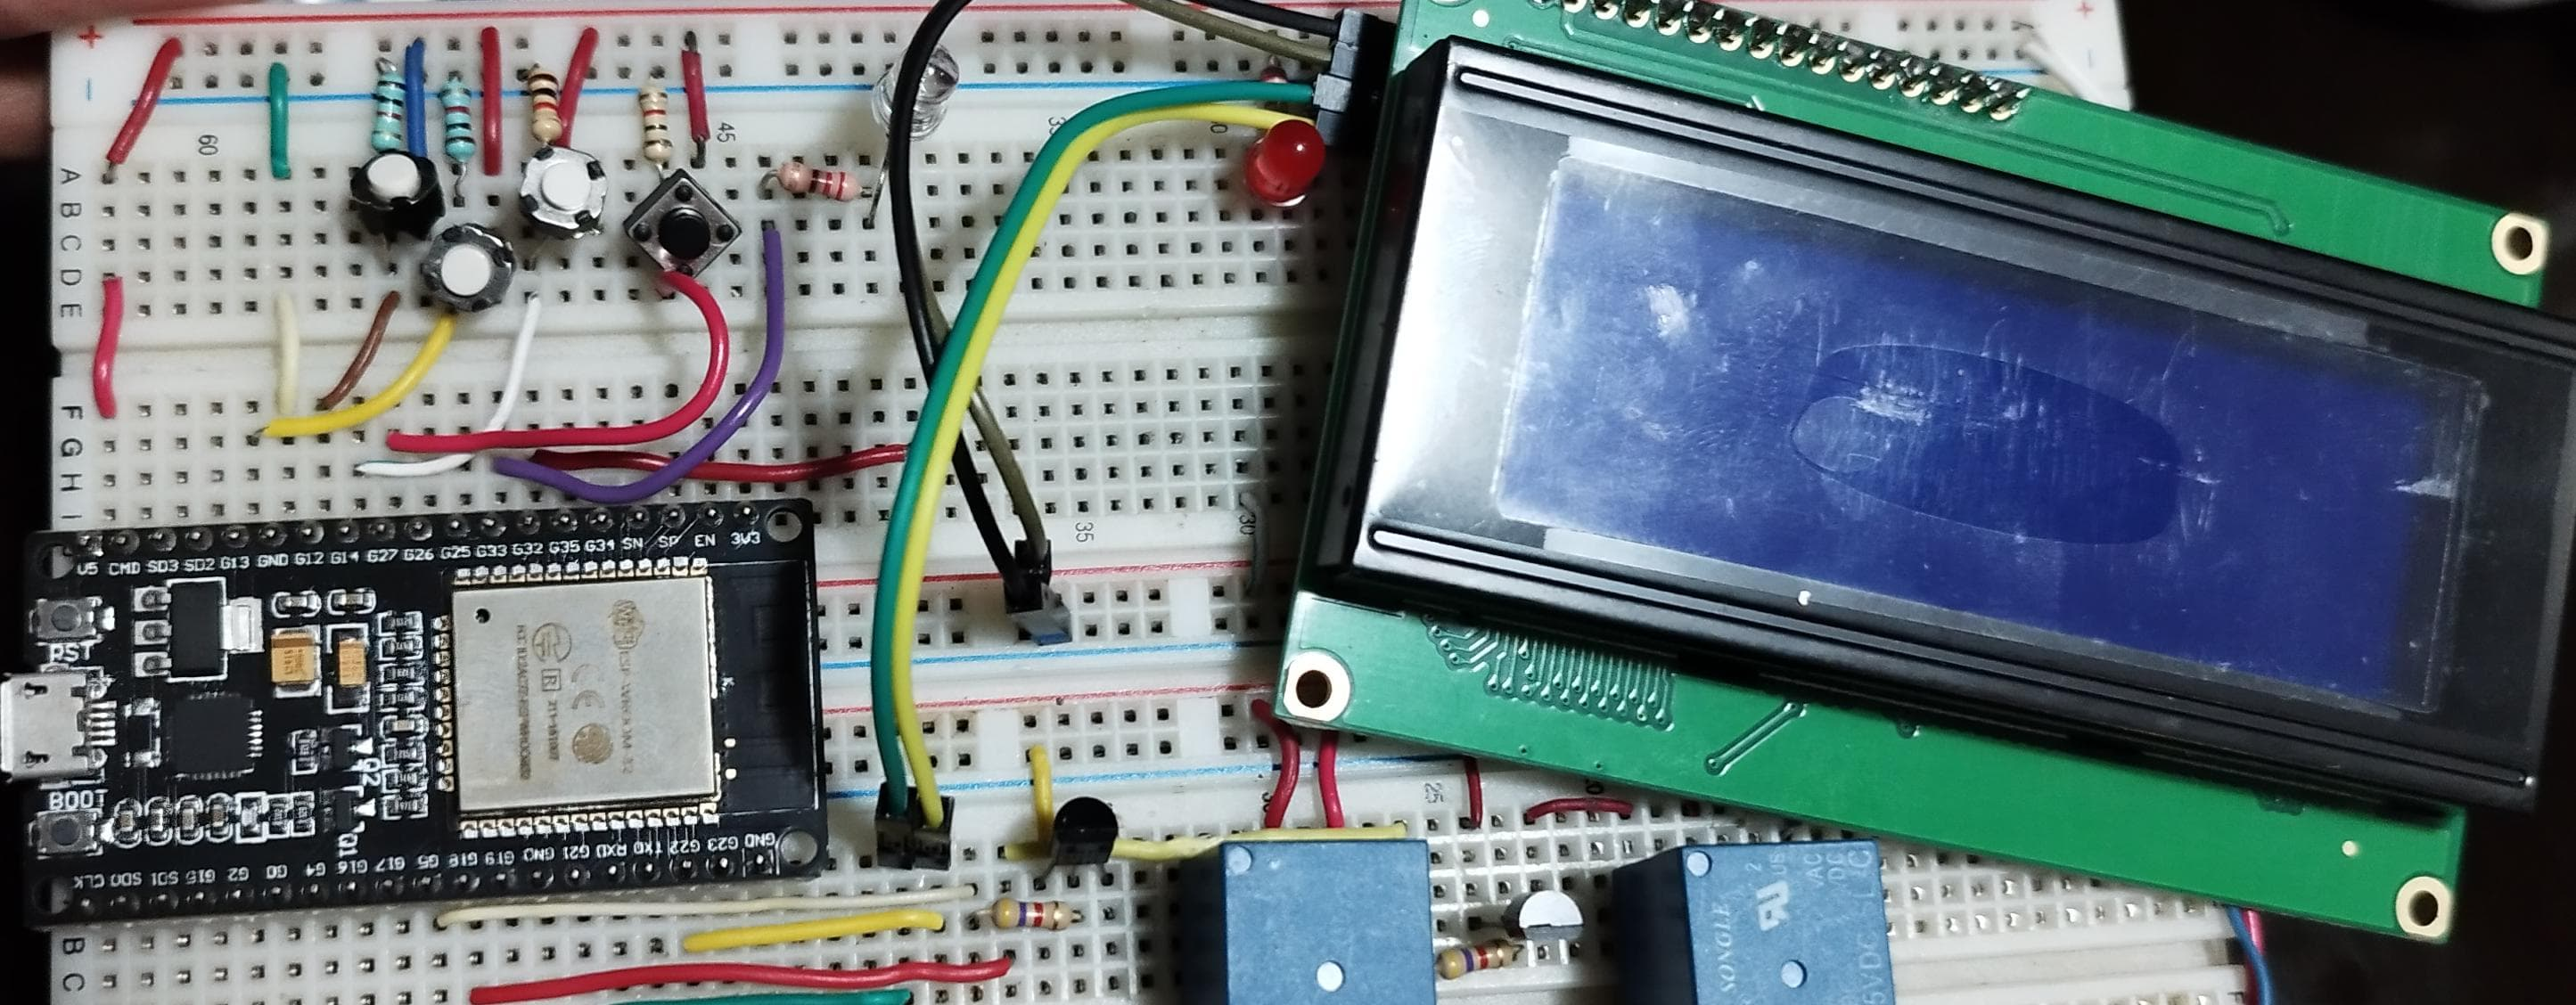
\includegraphics[scale=0.1]{images/Capitulo_Imple/S1/interfaz/cto_interfaz_imp.jpeg}
            \caption{Circuito de prueba de la interfaz}
            \label{fg:cto_interfaz_fisico}
        \end{figure}

\begin{figure}[h]
            \centering
            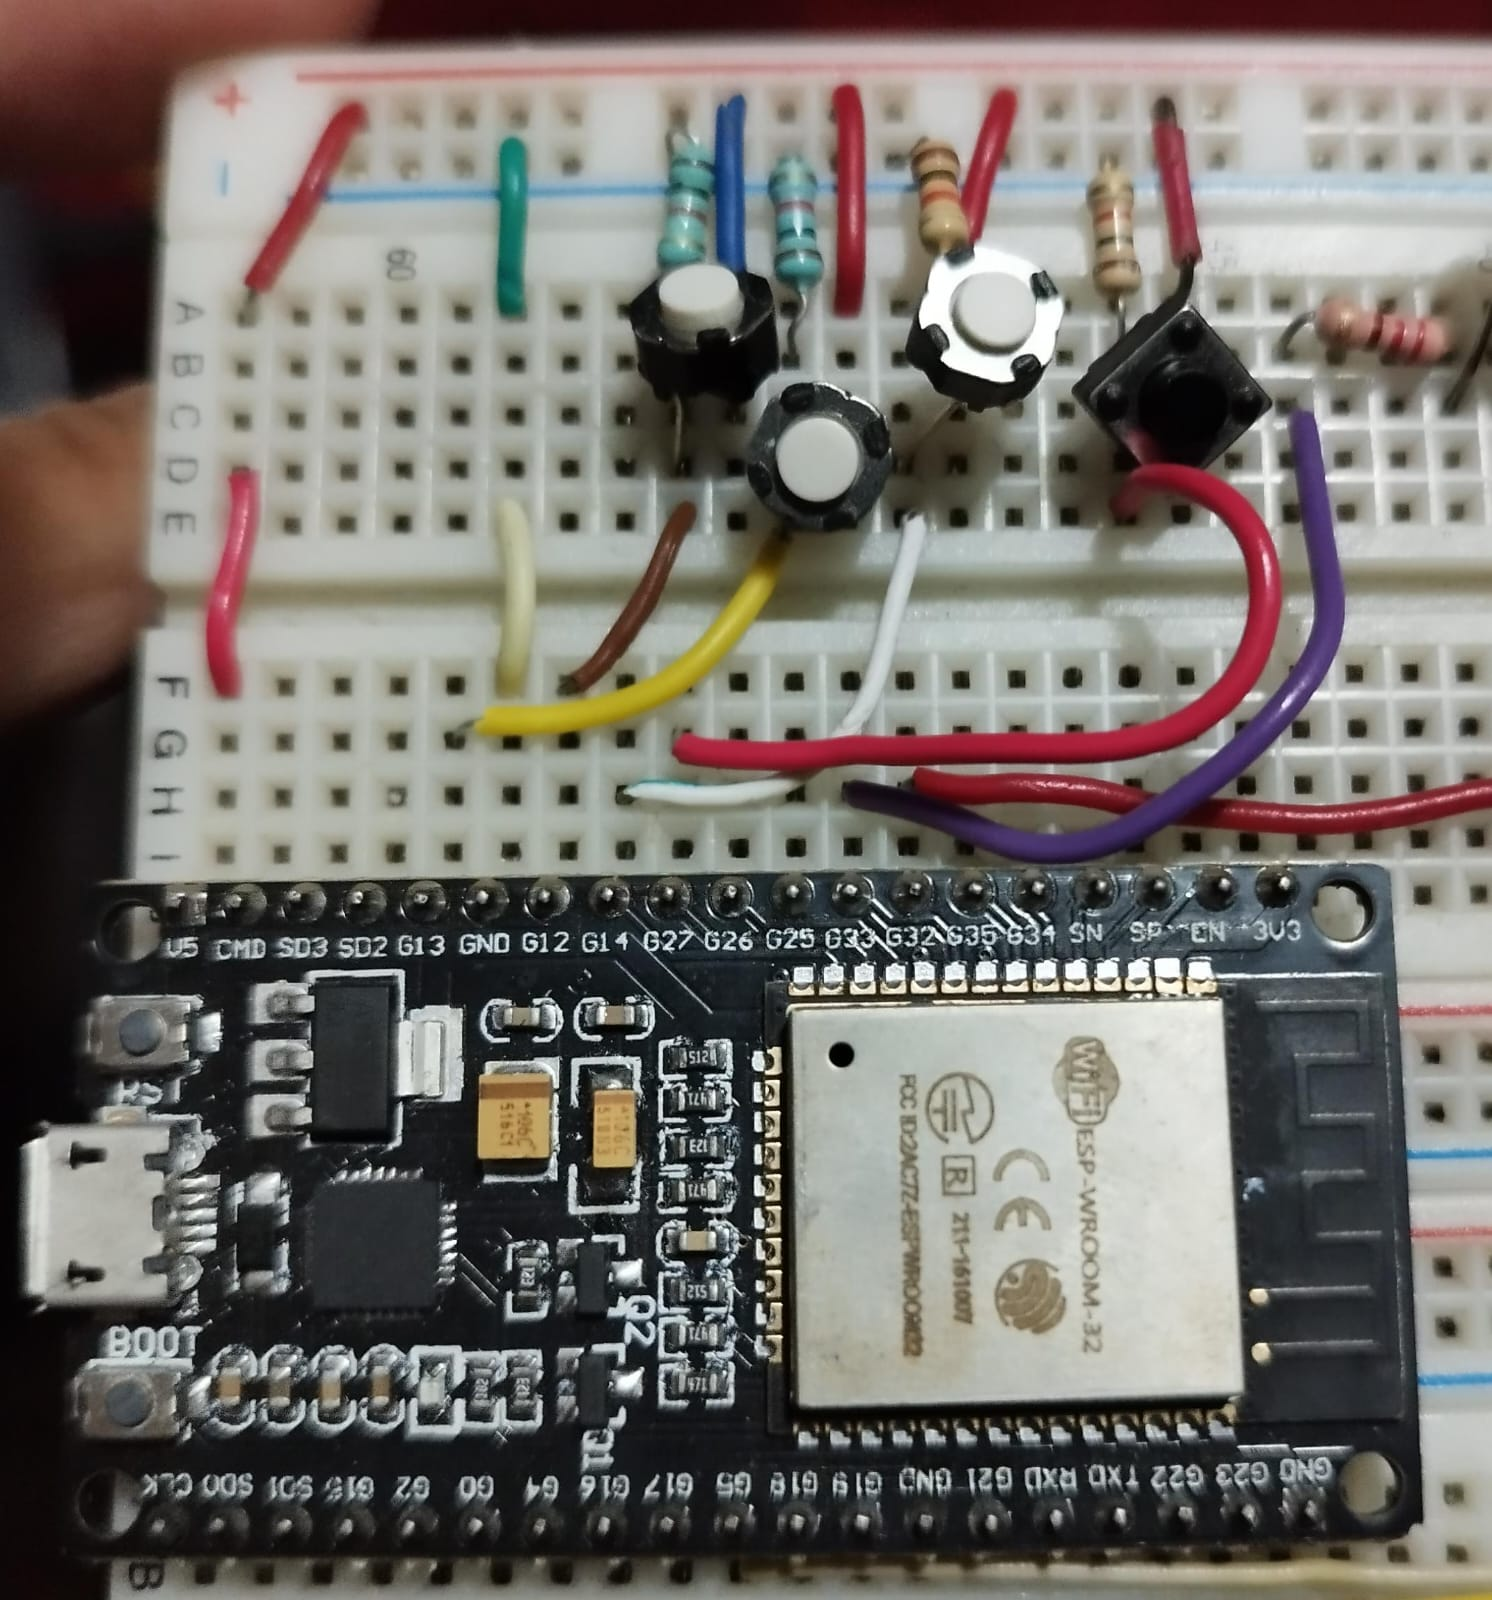
\includegraphics[scale=0.1]{images/Capitulo_Imple/S1/interfaz/botones_int.jpeg}
            \caption{Implementación de los botones}
            \label{fg:botones_imp}
        \end{figure}

\clearpage
Cada uno de los botones, representará cada una de las opciones que se presentarán en el menú (figura \ref{fg:menu_interfaz}) a través de la cual se podrá consultar información relevante acerca del ciclo de procesamiento del compost. Por ejemplo, los mensajes mostrados en las figuras \ref{fg:tiempo_proceso} y \ref{fg:proceso_en_ejecucion}.

\begin{figure}[h]
            \centering
            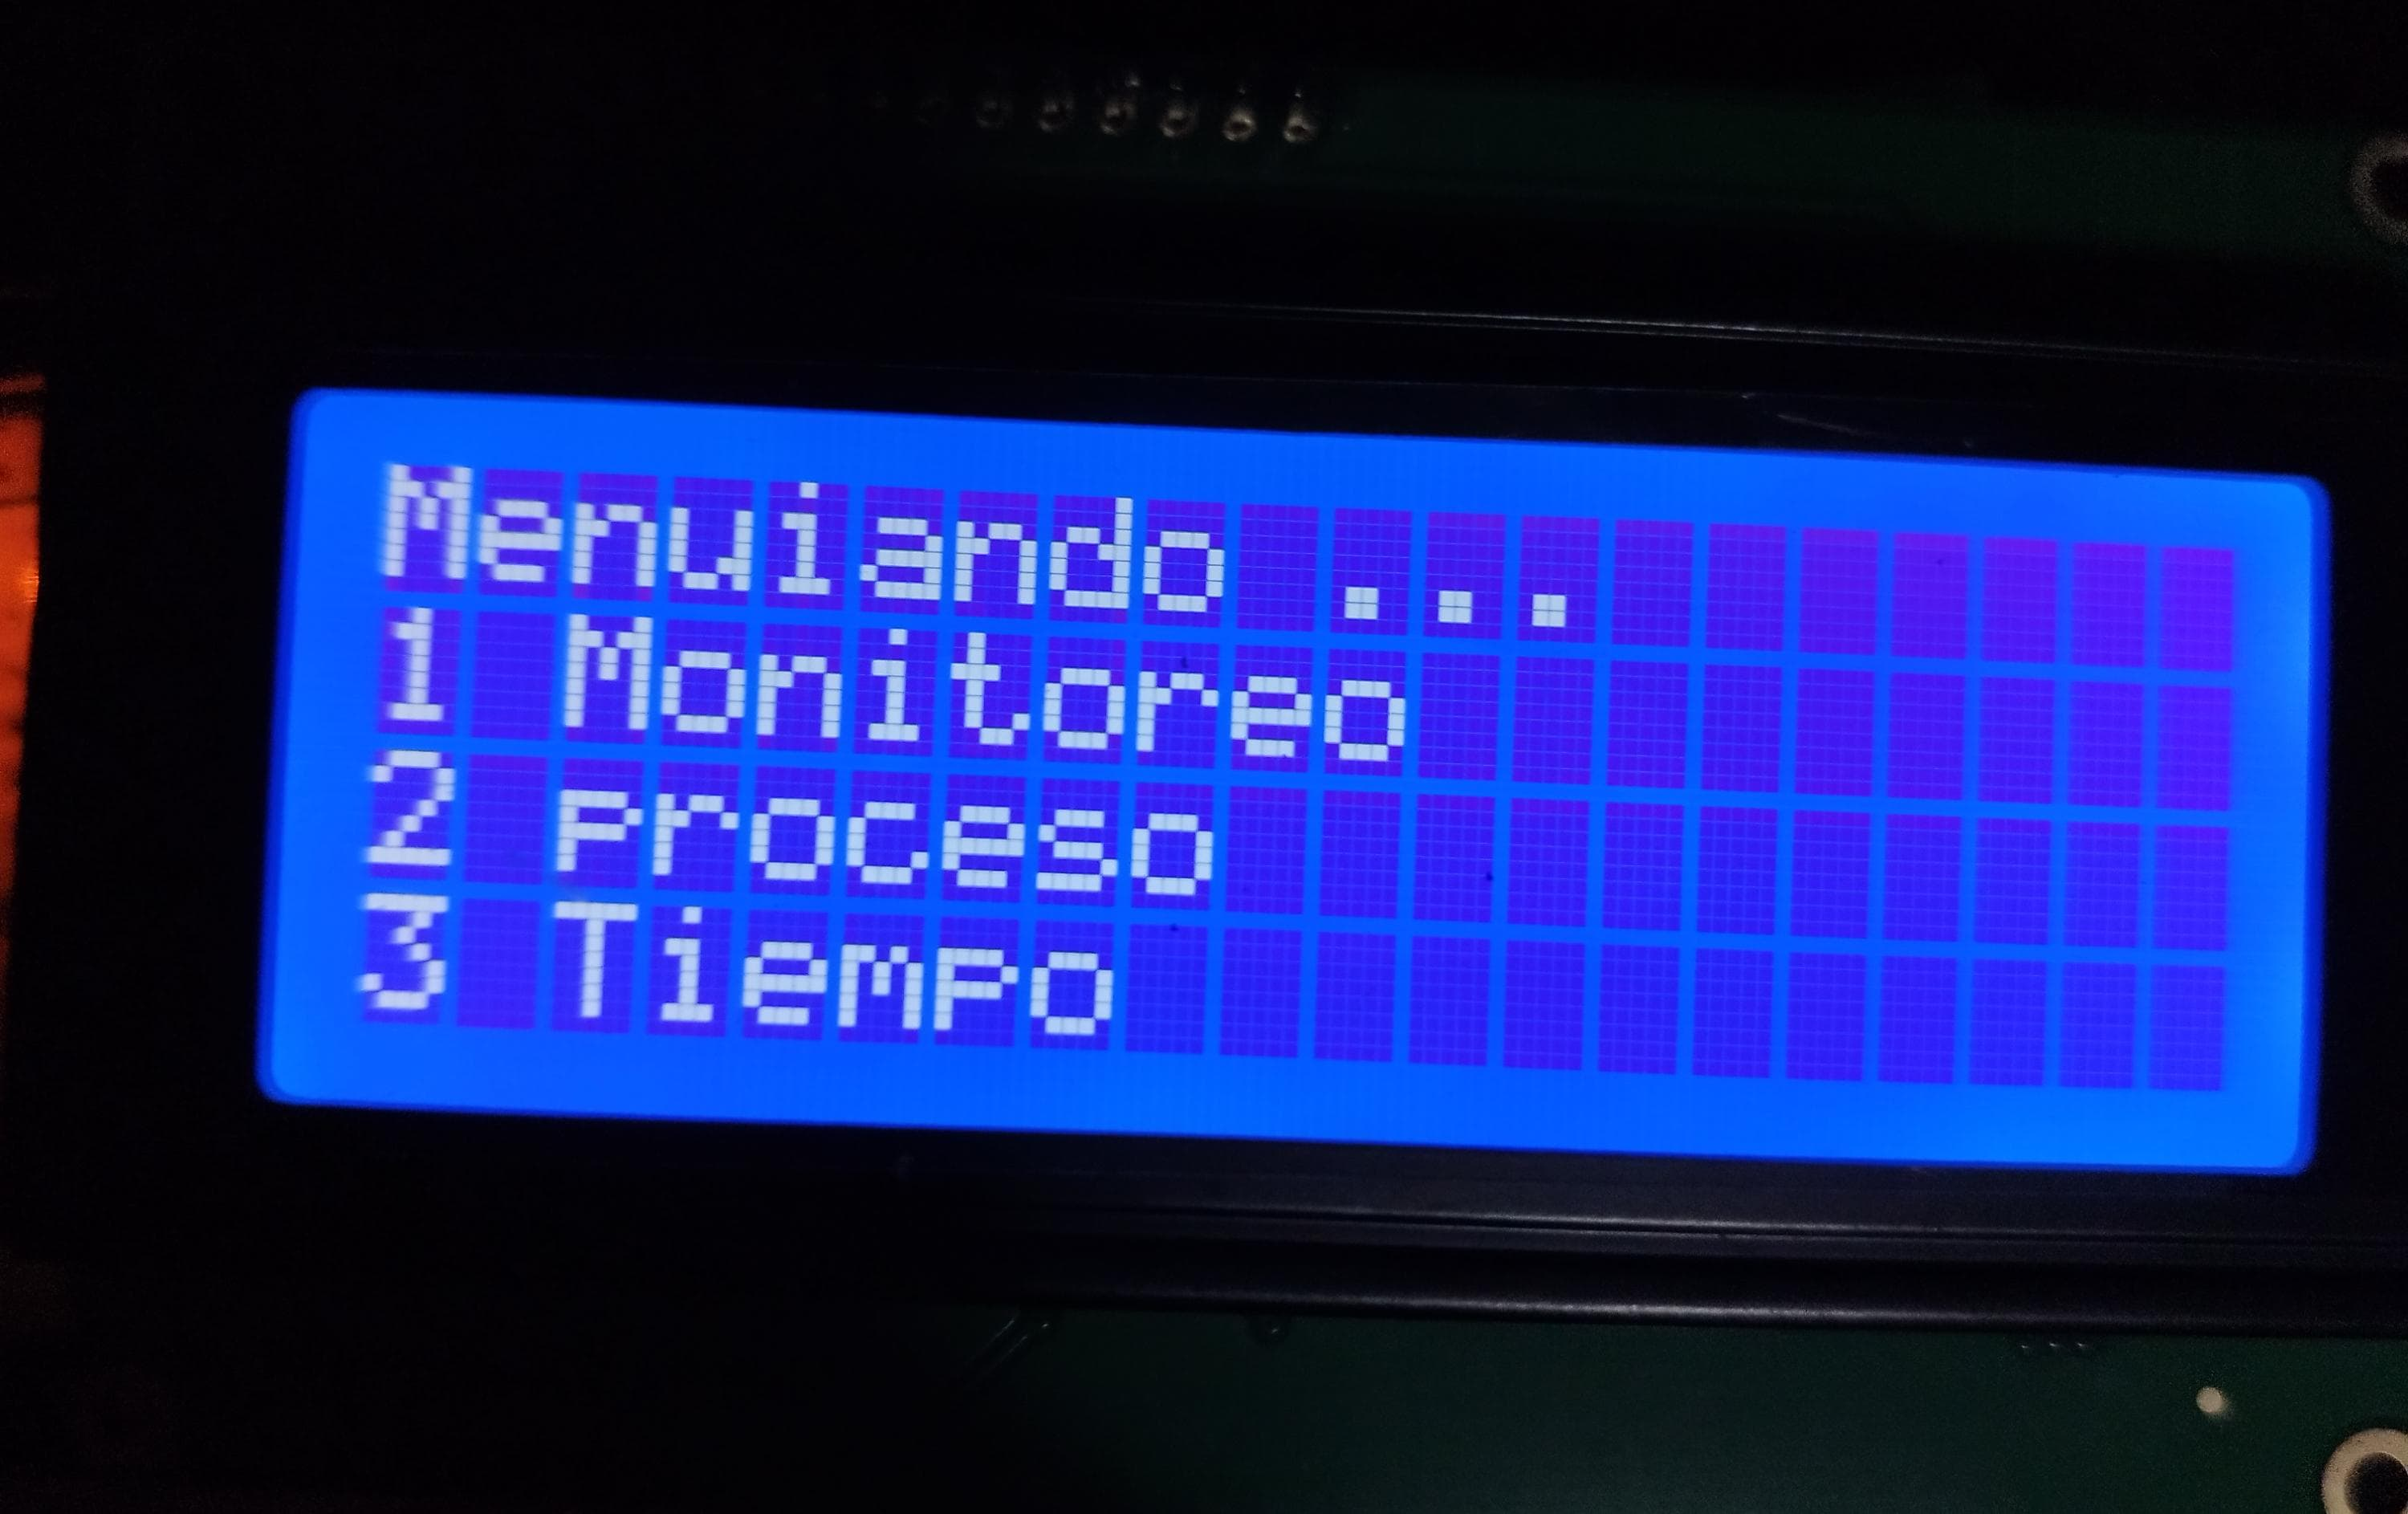
\includegraphics[scale=0.0555]{images/Capitulo_Imple/S1/interfaz/menu.jpeg}
            \caption{Menú desplegado por la interfaz}
            \label{fg:menu_interfaz}
        \end{figure}

\begin{figure}[h]
            \centering
            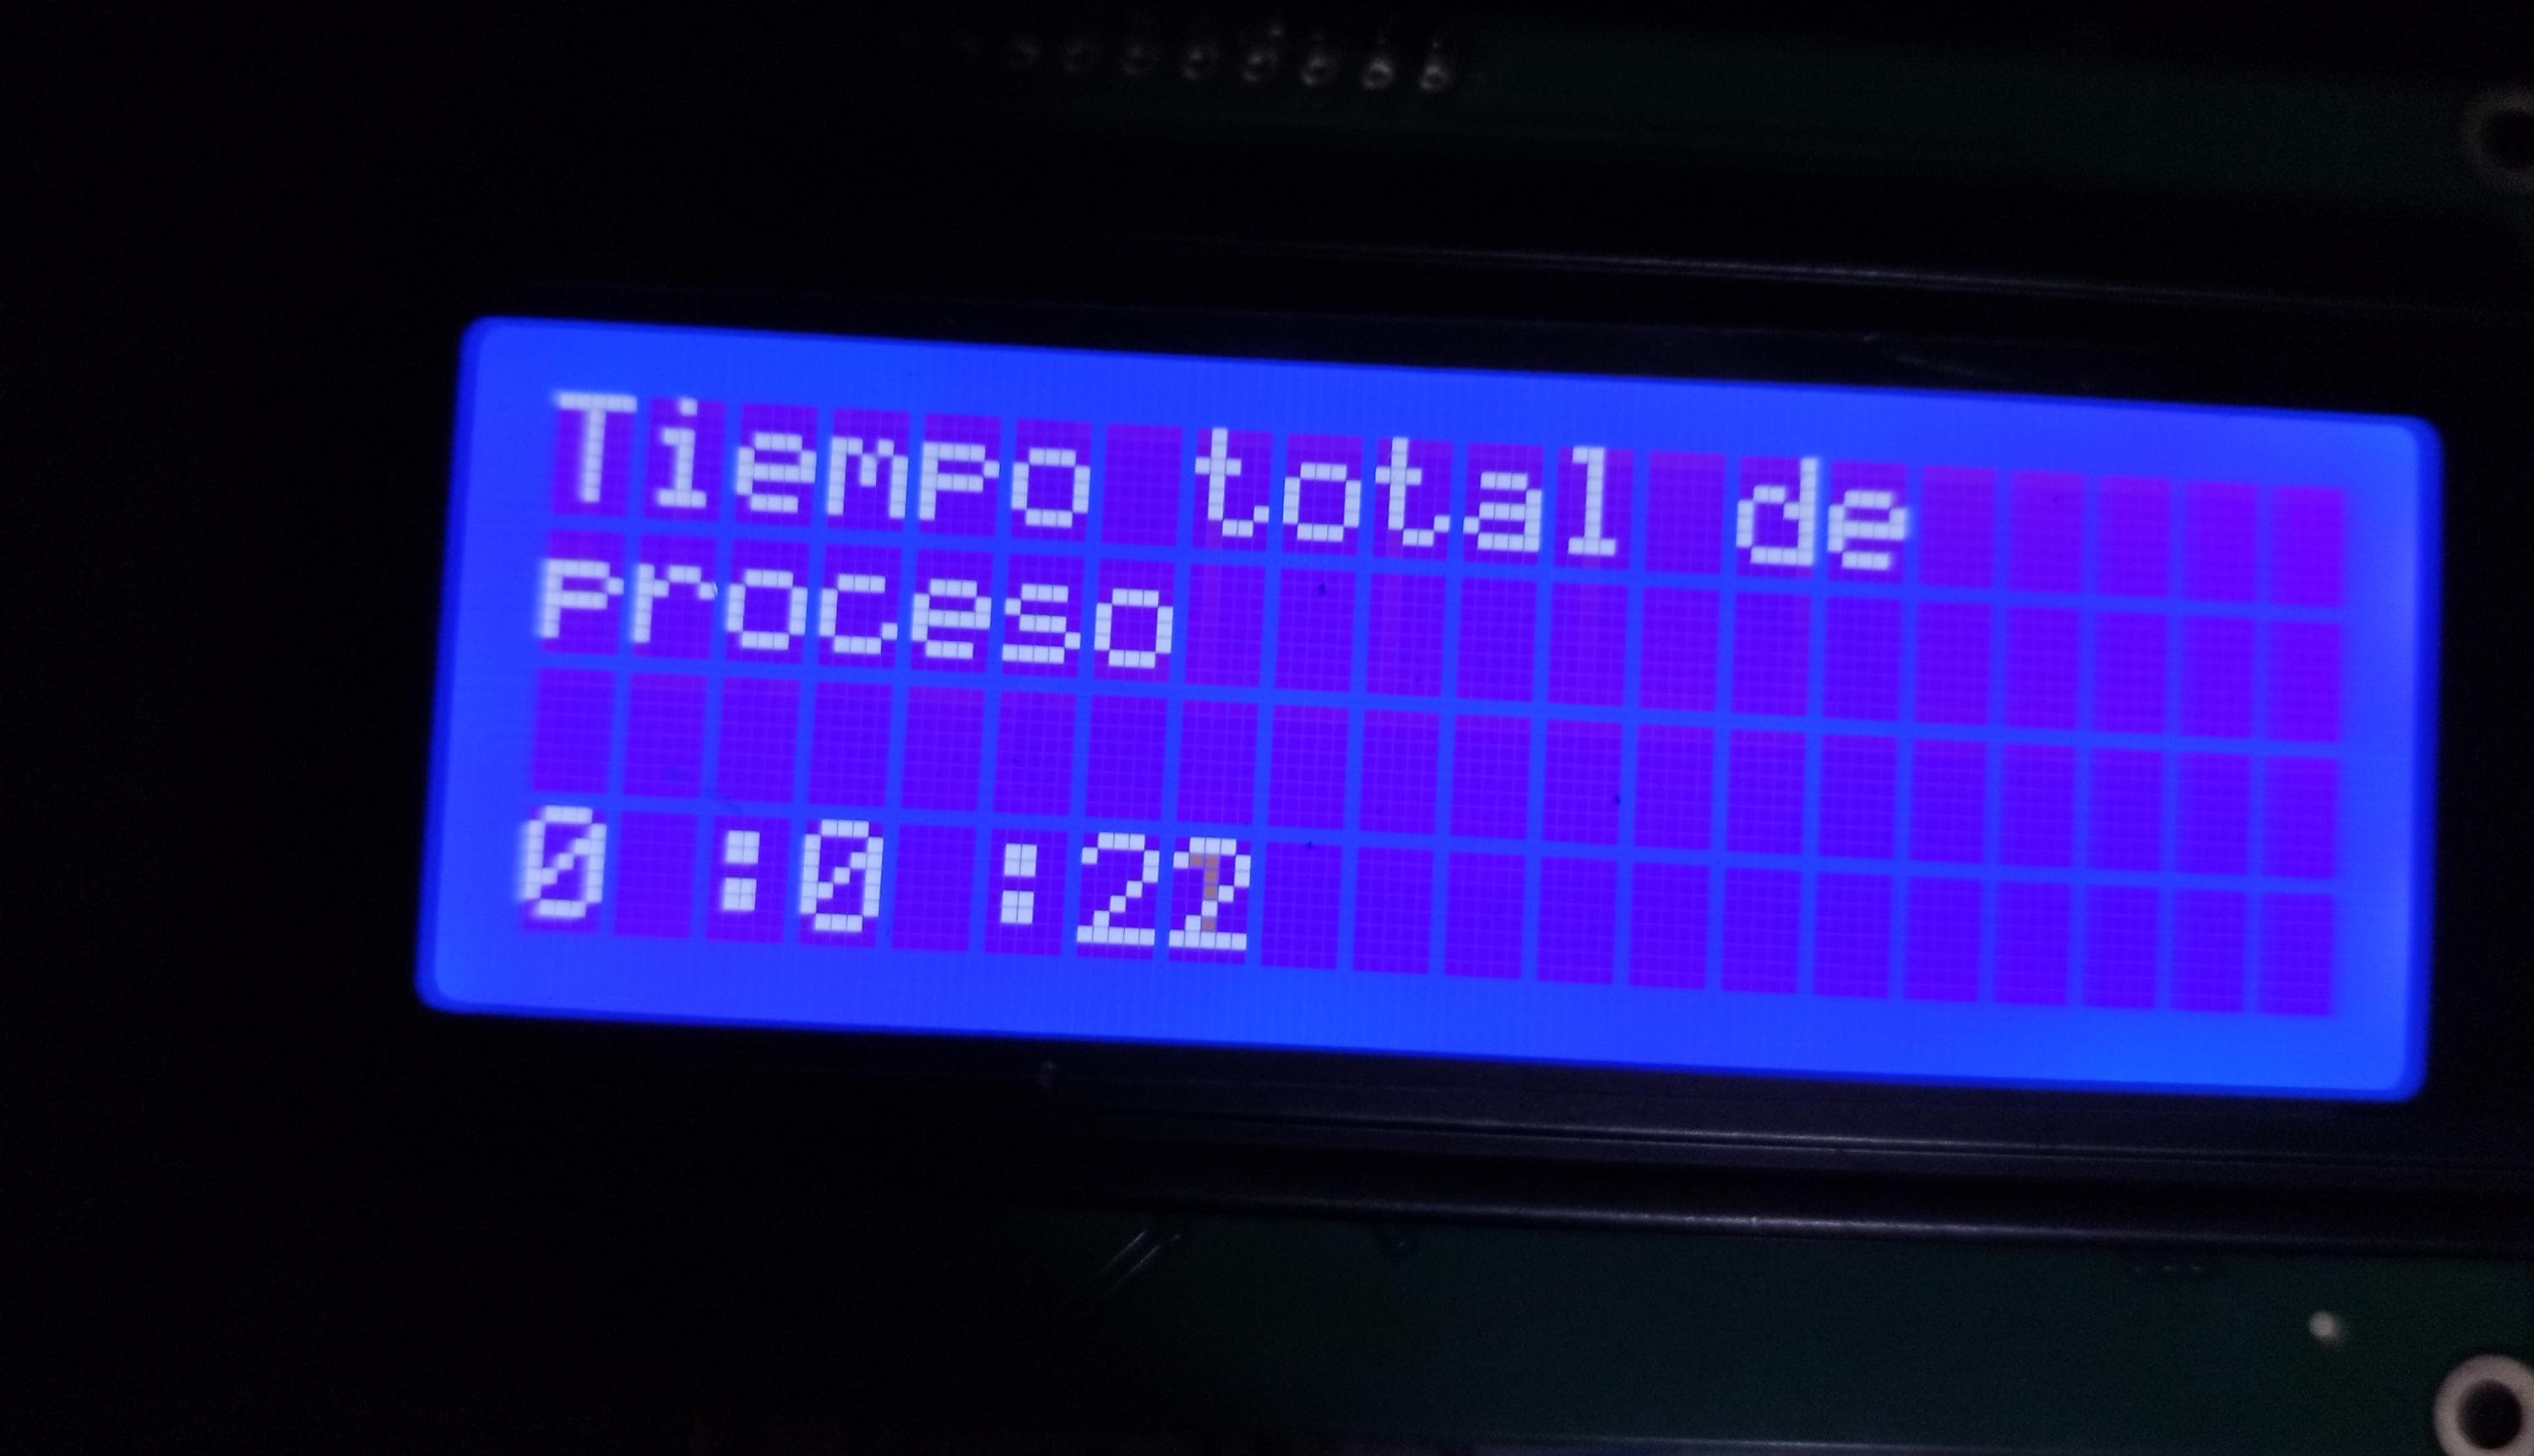
\includegraphics[scale=0.0555]{images/Capitulo_Imple/S1/interfaz/tiempo.jpeg}
            \caption{Representación del tiempo del proceso}
            \label{fg:tiempo_proceso}
        \end{figure}

\begin{figure}[h]
            \centering
            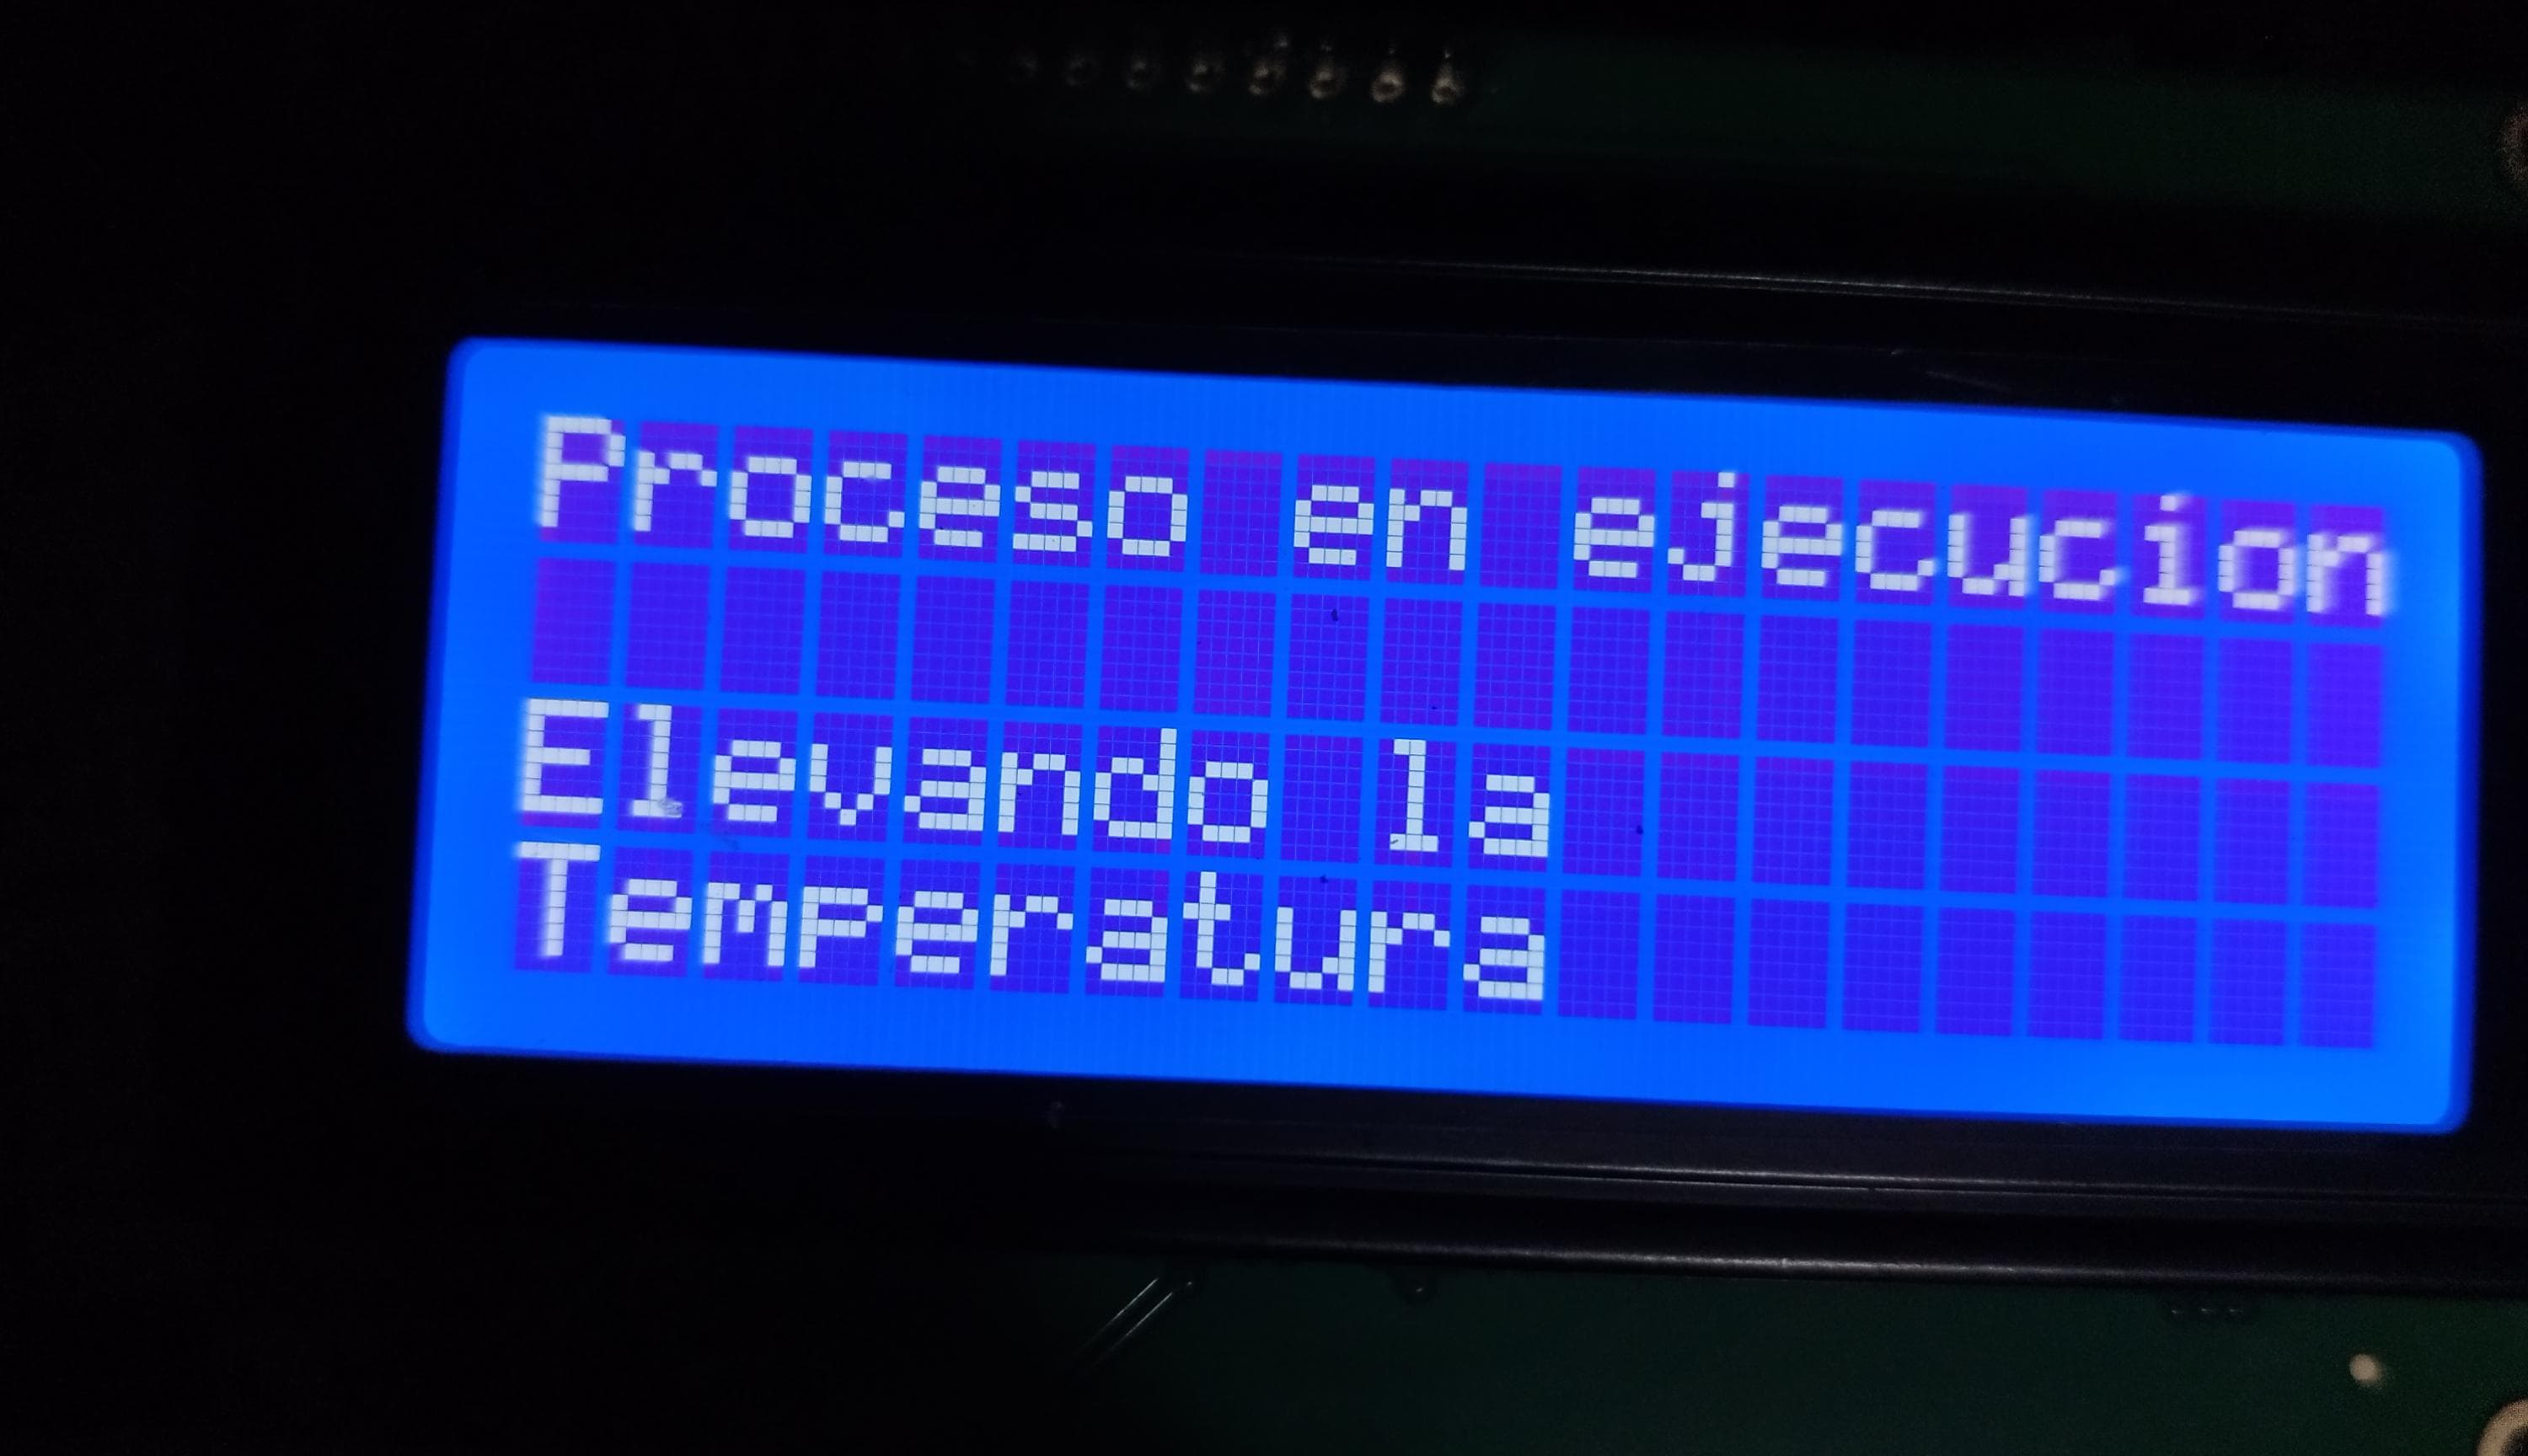
\includegraphics[scale=0.0555]{images/Capitulo_Imple/S1/interfaz/proceso.jpeg}
            
            \caption{Identificación del proceso en ejecución}
            \label{fg:proceso_en_ejecucion}
        \end{figure}
\textbf{Implementación monitoreo a distancia}
Durante la elaboración de este proyecto, se observó que la ESP32 es un microcontrolador bastante robusto y que posee distintas características, dentro de ellas se encuentra la conexión Wi-Fi. Buscando mejorar la experiencia del usuario se consideró que era posible monitorear el funcionamiento del dispositivo a distancia. Por tal motivo se propuso enviar las mediciones realizadas por los sensores a una pagina web para que el usuario pueda acceder de manera remota mediante un link y pueda observar el estado del dispositivo.
La página web para escritorio posee la siguiente distribución:
\begin{figure}[h]
            \centering
            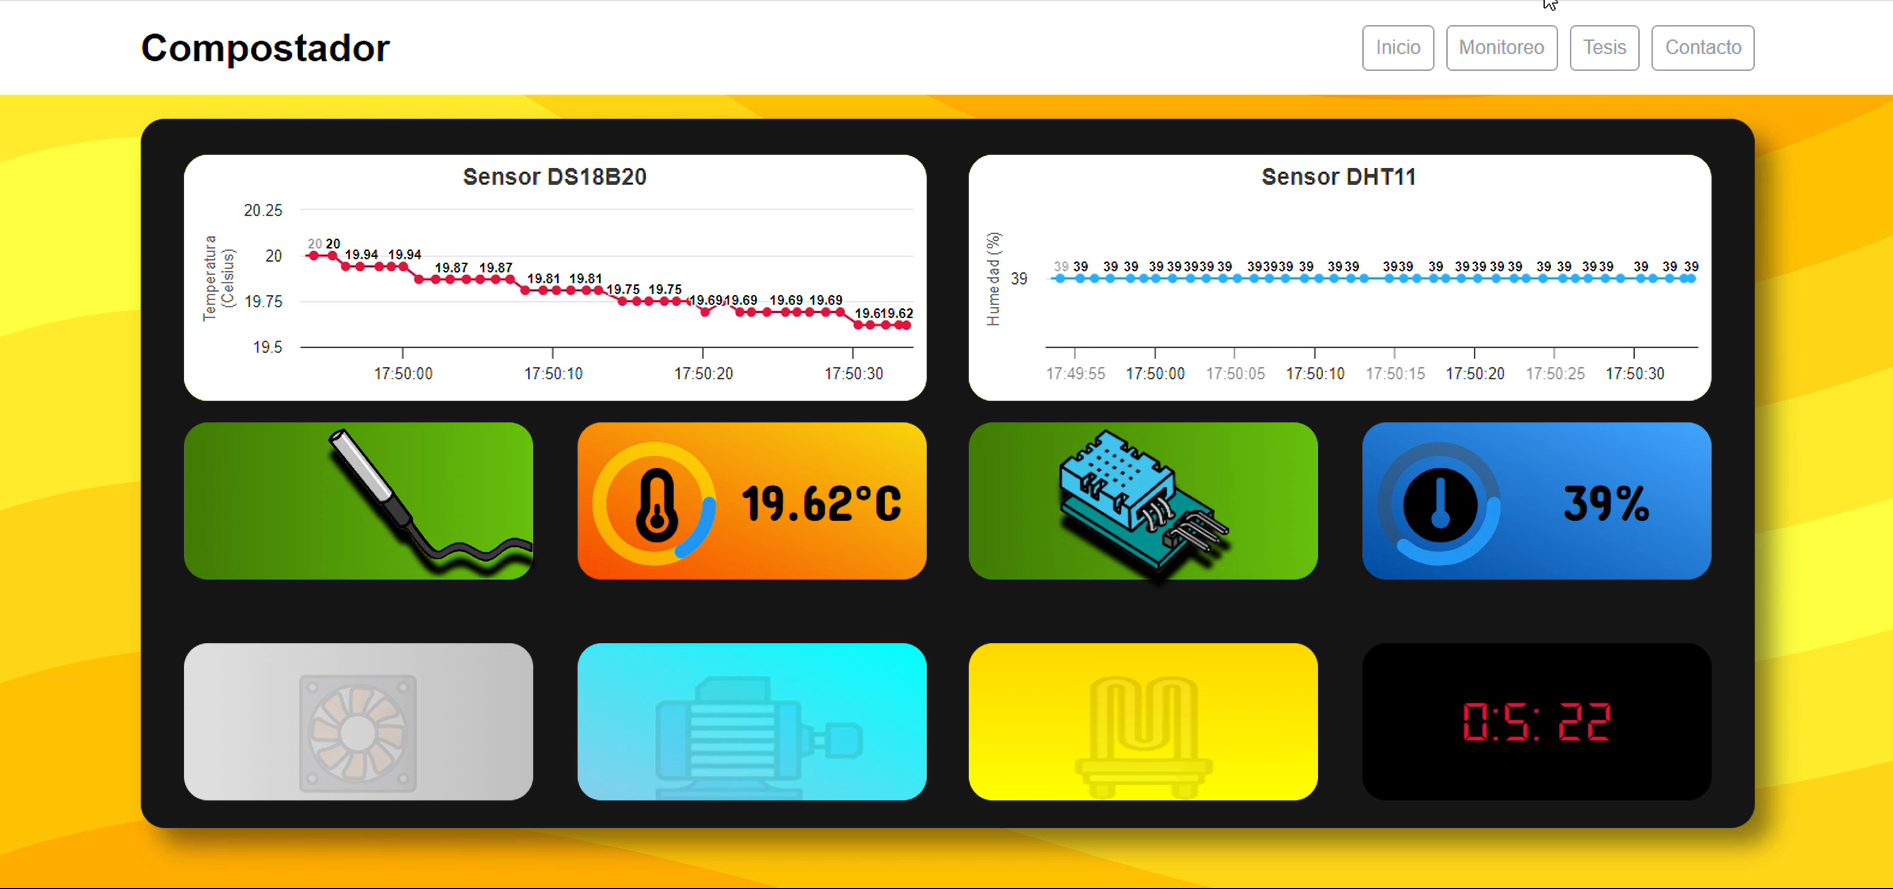
\includegraphics[scale=0.1]{images/Web/pagina_compostador.png}
            
            \caption{Página web compostador}
            \label{fg:pagina_web}
        \end{figure}
Partiendo de la parte superior, se presenta el estado de los sensores tanto de temperatura(DS18B20) como de humedad (DHT11). De primera mano se presenta una grafica con las últimas 40 mediciones enviadas cada segundo, esta gráfica se va actualizando. Sin embargo pensando en la posibilidad de que no todos los usuarios saben interpretar una gráfica, se propuso mostrar el valor de la temperatura  y la humedad en un formato sencillo como si se tratara de la lectura de un termómetro.

\begin{figure}[h]
            \centering
            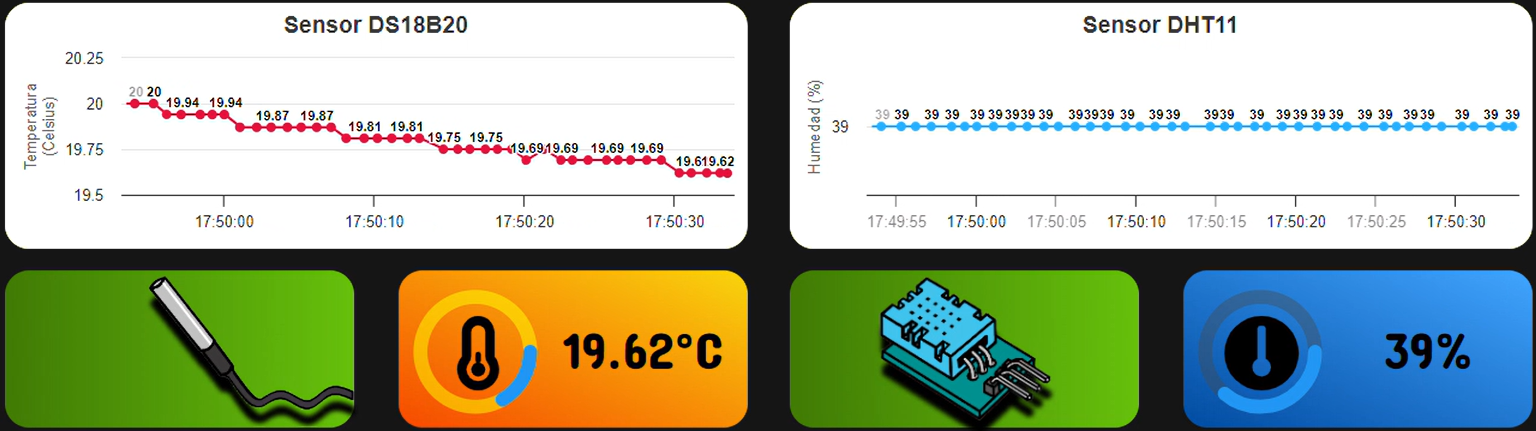
\includegraphics[scale=0.1]{images/Web/temp_hum_web.png}
            
            \caption{Estado sensor DS18B20 y DHT11}
            \label{fg:pagina_web}
        \end{figure}
                 Este indicador busca ser amigable con el usuario, se colocó un ícono de termómetro para que el usuario pueda asociarlo a la temperatura del sistema, el cual reacciona bajo ciertas condiciones previamente programadas ya que conforme este aumenta o disminuye la temperatura este reacciona a los cambios, por otro lado también se colocó un círculo que se va iluminando conforme la temperatura avanza en porcentaje. Conforme a los rangos de temperatura, este círculo cambia de color es decir, en un rango de temperatura mayor a los 0°C pero menor a los 20°C el circulo se iluminará de color azul cielo indicando al usuario una temperatura baja, cuando la temperatura es mayor de 20°C pero menor a 50°C el círculo se iluminará de color naranja y en temperaturas mayores a 50°C será rojo indicando alta temperatura.
            
                \begin{figure}[h]
               \centering
            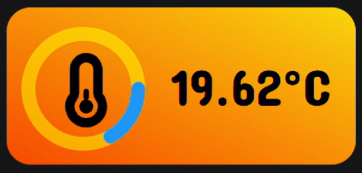
\includegraphics[scale=0.1]{images/Web/indicador.png}
            
            \caption{Indicador de temperatura baja}
            \label{fg:pagina_web}
        \end{figure}
\begin{figure}[h]
            \centering
            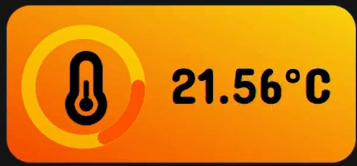
\includegraphics[scale=0.1]{images/Web/indicador_temp.png}
            
            \caption{Indicador temperatura media}
            \label{fg:pagina_web}
        \end{figure}
        Como en todo sensor existe la posibilidad de una falla en la lectura o de un daño en el componente, por lo que se propuso alertar al usuario cuando esto suceda.
        En el caso del sensor DS18B20 cuando este falle arrojará una medición de 0°C, además la casilla donde se encuentra representado el sensor, se iluminará de rojo, y en el indicador de temperatura el círculo se irá a cero así como el termómetro simulará no tener medición. 
\begin{figure}[h]
            \centering
            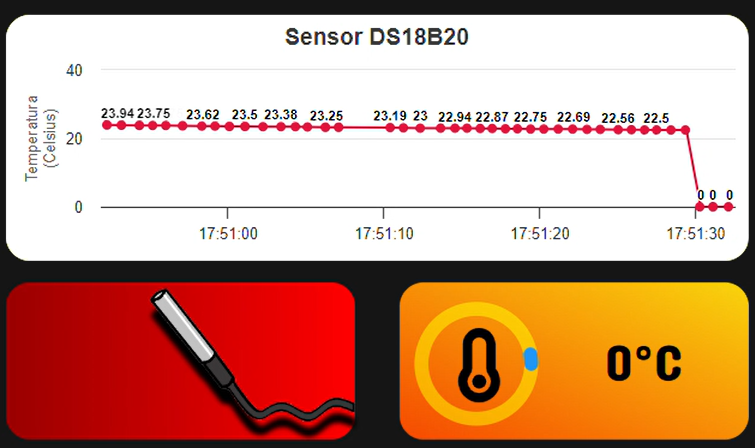
\includegraphics[scale=0.1]{images/Web/error_ds18.png}
            
            \caption{Error sensor DS18B20}
            \label{fg:pagina_web}
        \end{figure}
        En el caso del sensor de humedad, pasa algo similar, siendo que aquí se visualiza la lectura NaN\% (Not a Number) , de igual manera la casilla se iluminará de rojo y el indicador que simula un higrómetro analógico se irá a cero y el circulo también.
        \begin{figure}[h]
            \centering
            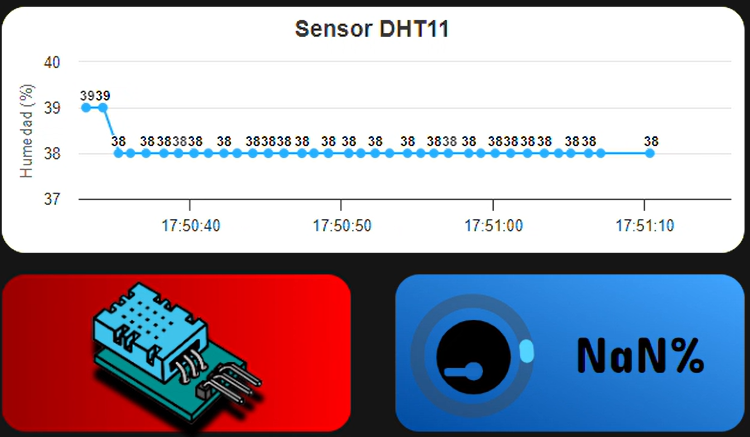
\includegraphics[scale=0.1]{images/Web/dht11_web.png}
            
            \caption{Error sensor DHT11}
            \label{fg:pagina_web}
        \end{figure}
Durante el proceso de compostaje se requiere activar algunos componentes como es el caso de un ventilador, un motor y el cinturón para calentar el tambo. Sin embargo saber que están activados podría ser útil para el usuario, por lo que cada que se enciende alguno de estos dispositivos, se ejecuta una animación que indica el estado de funcionamiento, cuando se apagan, la animación se detiene simulando un estado de pausa.
\begin{figure}[h]
            \centering
            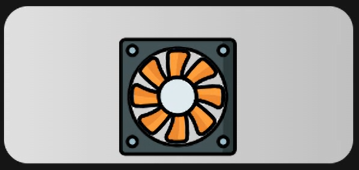
\includegraphics[scale=0.1]{images/Web/ventilador_web.png}
            
            \caption{Activación ventilador}
            \label{fg:pagina_web}
        \end{figure}
\begin{figure}[h]
            \centering
            
\includegraphics[scale=0.1]{images/Web/motor_web.png}
            
            \caption{Activación motor}
            \label{fg:pagina_web}
        \end{figure}
        \begin{figure}[h]
            \centering
            
\includegraphics[scale=0.1]{images/Web/resistencia_web.png}
            
            \caption{Activación resistencia}
            \label{fg:pagina_web}
        \end{figure}
        Por último para saber en qué punto del proceso se encuentra, se colocó un temporizador regresivo que mediante el almacenamiento local de la página registra la hora y aunque la pagina web se actualiza, el temporizador no se reinicia.
\begin{figure}[h]
            \centering
            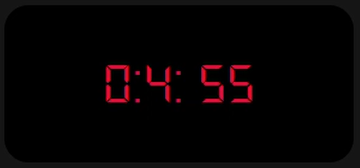
\includegraphics[scale=0.1]{images/Web/temporizador_web.png}
            
            \caption{Temporizador regresivo}
            \label{fg:pagina_web}
        \end{figure}
\begin{figure}[h]
            \centering
            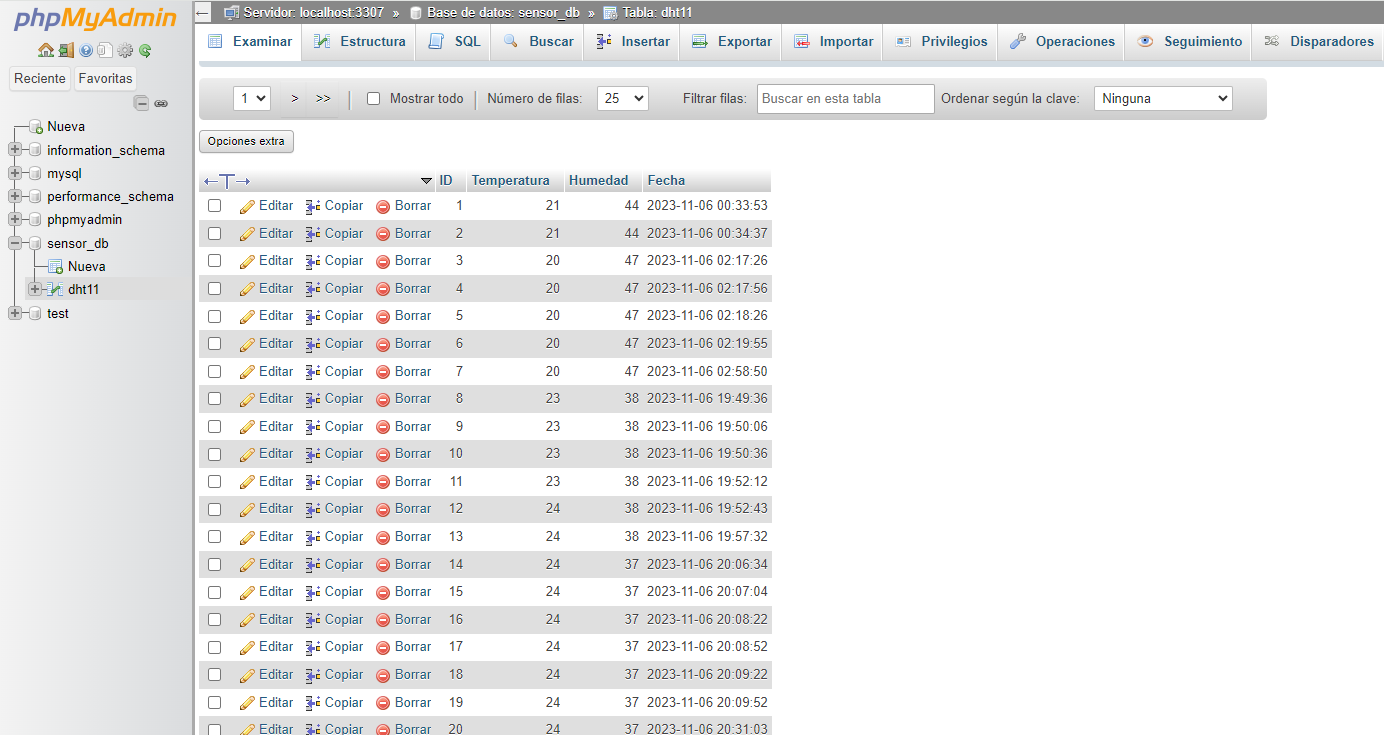
\includegraphics[scale=0.1]{images/Web/Db_compostador.png}
            
            \caption{Base de datos }
            \label{fg:pagina_web}
        \end{figure}
\clearpage